\section{Evaluation}
\label{ws:evaluation}
\paragraph{Setup.}
The main host has a Ryzen 7 255, approximately 44 GiB RAM, NVMe storage and an
RTX 5070 Ti with 16 GiB device memory. Software comprises Torch 2.11.0+cu128,
Triton 3.6.0, PyG 2.8.0.post1, pyg-lib 0.9.0+pt211cu128 and driver 595.84.
These are shared, non-clock-locked hosts. Timings are synchronized host wall
time through completed output. The comparisons use ordinary Torch inputs;
paging and distributed runs use native tensors. All performance results are
FP32 forward evaluations, not training steps. Figure~\ref{ws:performance}
shows matched shapes and semantics, with lower latency and allocation preferable.

\subsection{Generated and stored relations}
Stored CSR uses degree 32 and 32 features at 8,192--131,072 nodes. Baselines
are Torch sparse multiplication and PyG COO gather--scatter. Dynamic radius
uses a scalar distance-weighted sum, nominal degree 32 and the same node sizes.
Dynamic kNN uses a scalar neighbor sum with $k=16$ at 1,024--131,072 points.
Each dynamic call changes coordinates, constructs the relation and consumes
it; unchanged-input topology caching is not timed as construction.

PyG baselines use their respective radius/kNN builder plus COO message passing.
Pure Torch baselines compute distances in bounded row chunks and then use
CSR/sparse multiplication for radius, or top-k followed by gather/sum for kNN.
The distance-block budget is 16,777,216 pairs. These eager all-pairs baselines
do not represent the best possible spatial-index implementation in Torch.
Complete explicit-reference/PyG edge sets agree for both coordinate snapshots.
Radius inputs avoid ambiguous floating-point cutoffs, and the neighbor cap
does not truncate the measured relations.

Each of 36 configurations runs in a fresh process, with provider order
randomized, four warmups and ten timed calls checked at relative and absolute
tolerance $3\cdot10^{-4}$. Curves show medians and sample ranges. Peak
Torch-allocated bytes include inputs, output, graph representations and
temporaries, but exclude allocator reserve, CUDA context and other processes.
Largest-shape audits found no extra Tiga-native device-buffer allocation on
these Torch paths. Compilation is outside the warm timing window.

\begin{figure}[t]
\centering
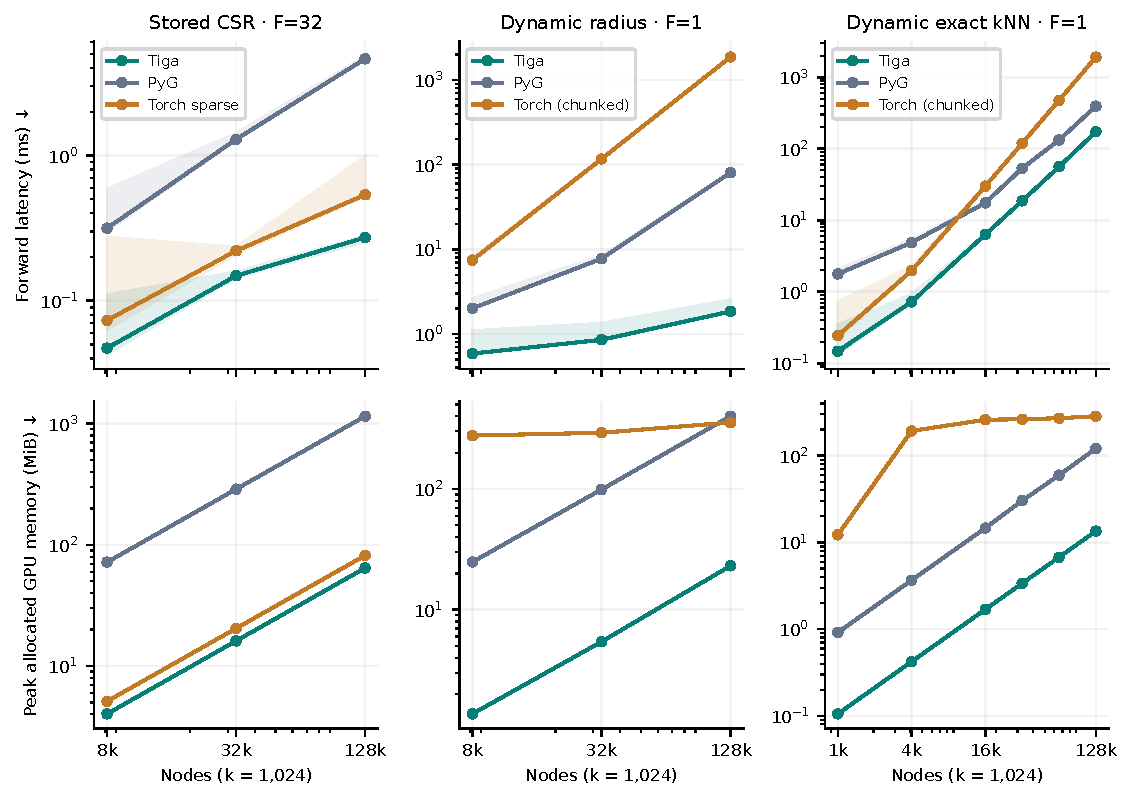
\includegraphics[width=\linewidth]{figures/q1-performance-memory.pdf}
\caption{Matched forward latency and allocated GPU memory. Columns are distinct
workloads: stored CSR has 32 features, dynamic radius and kNN have one.
Both axes are logarithmic. Dynamic calls include rebuilding from changed
coordinates; Torch (chunked) uses a pure Torch builder and aggregation.}
\label{ws:performance}
\end{figure}

Stored CSR achieves 1.49--1.97$\times$ speedup and approximately 1.27$\times$
lower allocation than Torch sparse across the three sizes. At 131,072 radius
points, Tiga takes 1.84 ms versus 80.24 ms for PyG and 1,870.09 ms for chunked
Torch, with allocation of 23.14, 400.22 and 355.01 MiB respectively. This
comparison combines algorithmic traversal choices and materialization/fusion
effects; it does not isolate the contribution of any one compiler pass.

At 131,072 kNN points, Tiga takes 172.37 ms versus 393.21 ms for PyG and
1,908.43 ms for chunked Torch; the allocations are 13.50, 121.13 and 285.00 MiB.
The PyG-relative speedup ranges from 2.28$\times$ to 12.06$\times$ over six
sizes. These results concern scalar messages on the tested geometries, not
wide-feature EdgeNNs or arbitrary point distributions.

\subsection{Billion-edge capacity and its cost}
The capacity workload explicitly stores a periodic directed CSR graph with
16 neighbors per destination and 32 features. The sweep contains 10M, 100M
and 1B edges with three fresh-process calls per size. Ingest is excluded;
forward includes loading, staging, compilation as encountered, computation
and output assembly. All output values are checked after timing against a
closed-form oracle; the execution still traverses every stored edge.

Pages contain 65,536 destination rows, the managed-device budget is 12 GiB,
and prefetch is disabled. At 1B edges, the graph has 62.5M nodes. Int64 CSR,
source and output together require at least 22.82 GiB for full residency
(18.86 GiB with int32 CSR), exceeding device capacity. These are calculated
lower bounds, not measured baseline OOMs.

\begin{figure}[t]
\centering
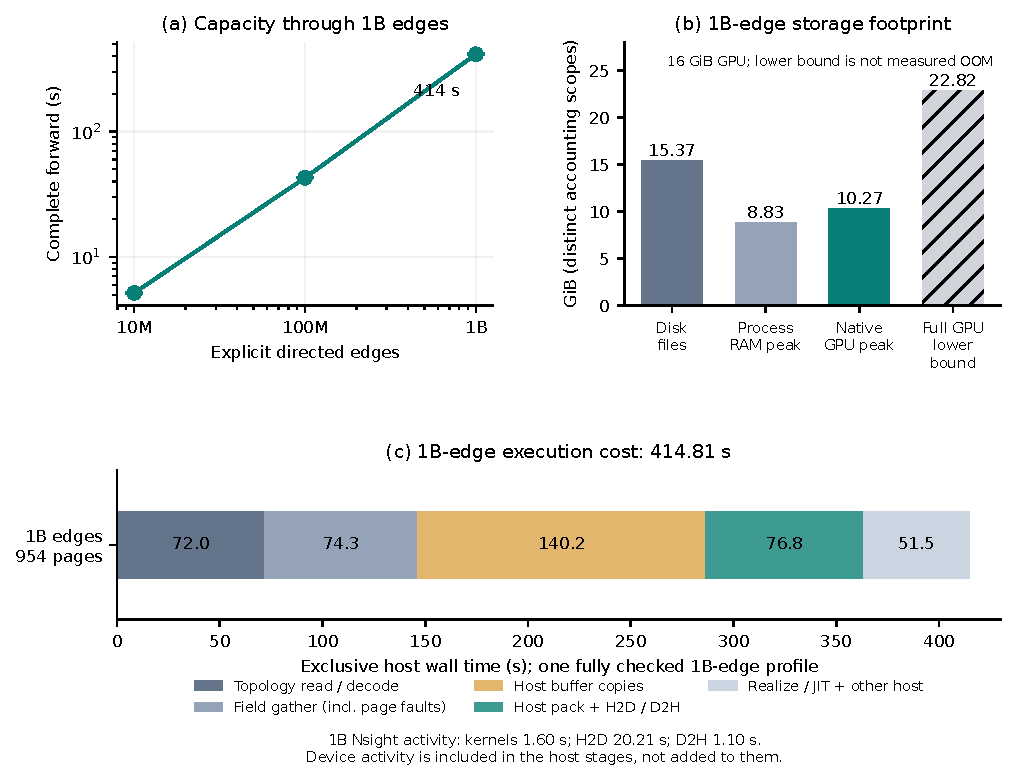
\includegraphics[width=\linewidth]{figures/q2-capacity-cost.pdf}
\caption{Capacity through 1B explicit edges. The full-residency requirement is
calculated; other memory bars have distinct measured accounting scopes.
The host-stage breakdown is one separately instrumented forward call, not
extra time added to the three-trial capacity sweep.}
\label{ws:capacity}
\end{figure}

The 1B median is 414.25 s (411.36--415.61), with maximum native GPU peak
10.27 GiB and forward process RSS 8.83 GiB. Disk topology/source storage is
15.37 GiB, and the resident output alone is 7.45 GiB. Sampled device-wide
usage, including unrelated services and pools, reaches 13.25 GiB.

A separate checked 1B profile spends 414.81 s in its forward window:
71.98 s topology read/decode, 74.27 s field gathering, 140.22 s host-buffer
copying, 76.79 s packing/transfers and 51.55 s setup/assembly/other work.
Nsight records 1.60 s of CUDA kernels and 20.21 s H2D activity inside those
host intervals. Source expansion turns 8 GB of stored features into 128 GB
of gathered values. Host staging, not reduction arithmetic, dominates.
The result establishes execution beyond device memory, not optimal offload
performance, capacity beyond host RAM, or a maximum supported edge count.
A hand-chunked peer could also trade storage traffic for capacity.

\paragraph{Distributed scope.}
For a separate two-host spatial-mesh experiment, a 5070 Ti and 4070 Ti SUPER
each own half the destination rows and exchange a one-layer halo through
NCCL Socket transport before local computation. At 22.51M directed edges,
paired-rank latency is 44.22 ms, versus 23.00 ms on the faster GPU alone.
Thus the current fixed partition does not establish a distributed speedup,
despite only 1.125 MiB of halo traffic. Appendix~\ref{ws:distributed} gives
the timing conditions and interpretation.
\FloatBarrier
